\documentclass{report}
\usepackage[utf8]{inputenc}
\usepackage{graphicx}
\usepackage[T1]{fontenc}
\usepackage{inconsolata}
\usepackage{appendix}
\usepackage[colorlinks=true, allcolors=black]{hyperref}



\usepackage{color}

\definecolor{pblue}{rgb}{0.13,0.13,1}
\definecolor{pgreen}{rgb}{0,0.5,0}
\definecolor{pred}{rgb}{0.9,0,0}
\definecolor{pgrey}{rgb}{0.46,0.45,0.48}

\usepackage{listings}
\lstset{language=Java,
  showspaces=false,
  showtabs=false,
  breaklines=true,
  showstringspaces=false,
  breakatwhitespace=true,
  commentstyle=\color{pgreen},
  keywordstyle=\color{pblue},
  stringstyle=\color{pred},
  basicstyle=\ttfamily,
  moredelim=[il][\textcolor{pgrey}]{$$},
  moredelim=[is][\textcolor{pgrey}]{\%\%}{\%\%}
}

\begin{document}

\begin{center}
    \huge \textbf{Gymnázium, Praha 6, Arabská 14}\\
    \Large předmět Programování, vyučující Mgr. Jan Lána   
\end{center}


\begin{figure}[h!]
    \centering
    
\includegraphics{images/GyarabRP.png}
    \label{fig:GyarabRP}
\end{figure}

\begin{center}
    \huge \textbf{Ročníková práce\\
    \Large Generátor Sudoku}\\
    \Large \textbf{Ivan Merkulov 1.E}\\
    Duben 2022
\end{center}


\chapter*{Čestné prohlášení}
\large Prohlašuji, že jsem jediným autorem tohoto projektu, všechny citace jsou řádně označené a všechna použitá literatura a další zdroje jsou v práci uvedené. Tímto dle zákona 121/2000 Sb. (tzv. Autorský zákon) ve znění pozdějších předpisů uděluji bezúplatně škole Gymnázium, Praha 6, Arabská 14 oprávnění k výkonu práva na rozmnožování díla (§ 13) a práva na sdělování díla veřejnosti (§ 18) na dobu časově neomezenou a bez omezení územního rozsahu.\\
\\
V Praze dne  ..........\hspace{3cm}..........................\hspace{1cm}..............

\chapter*{Abstrakt}
Cílem projektu je vygenerovat hru sudoku podle všech jeho základních pravidel. To znamená, že musíme zaplnit sudoku čísly, tak že v každém řádku, sloupci a čtverci musí být každé číslo právě jednou. Program je schopen vygenerovat sudoku o velikosti mřížky 4x4, 6x6 a 9x9, dokáže určit 3 stupně obtížnosti hry sudoku (Lehká, Střední, Těžká) a potom hru sudoku graficky zobrazí.

\chapter*{Abstract}
The aim of the project is to generate a sudoku game according to all its basic rules. This means that we have to fill the sudoku with numbers, so that each row column and square must have each number exactly once. The program is able to generate sudoku game grid of 4x4, 6x6 and 9x9 sizes, it also can determine 3 levels of difficulty of the sudoku game (Easy, Medium, Hard) and then graphically display the sudoku game.


\renewcommand{\contentsname}{Obsah}
\tableofcontents

\chapter{Úvod}
Sudoku je logická hra s číslicemi. Cílem hry v základní podobě je doplnit chybějící cifry 1-9 v zadané, zčásti vyplněné čtvercové mřížce s 9×9 poli. V tabulce jsou zvýrazněny 4 příčky vymezující 9 čtverců (3×3). K předem vyplněným číslicím je třeba doplnit další číslice tak, aby platilo, že v každém řádku, v každém sloupci a v každém z 9 čtverců 3x3 jsou použity vždy všechny číslice 1-9 a každá právě jednou. Tento dokument se zabívá generátorem náhodného řešitelného sudoku. Generátor dokáže vygenerovat sudoku různé velikosti a různé obtížnosti. Program je napsán v programovacím jazyce Java a grafické okno se vykresluje pomocí knihovny Swing. K řešení problému jsem přistoupil, tak že nejdříve by se vyplnila mřížka sudoku všemi čísly a potom by se náhodně vymazali čísla z mříšky, abychom jsme dostali hotový hlavolam. Při ukázce kódů budu dávat jako příklad kódy ke generování sudoku 9x9 pro jiné velikosti by stačilo zaměnit hodnotu 9 jinou příslušnou hodnotou (4, 6).\\
\\
\begin{Large}
\textbf{Zadání}\\
\\
\end{Large}
Zadání mé ročníkové práce bylo:\\
\\
1. Vygenerování náhodného řešitelného sudoku\\
2. Vygenerování různé velikosti sudoku\\
3. Vygenerování sudoku různé obtížnosti
\chapter{Zaplnění mřížky čísly}
Pro zaplnění mřížky všemi čísly dle pravidel sudoku, jsem použil dva způsoby.

\section{Řešení 1}
Řešení číslo 1 spočívá v tom, že budeme různě upravovat a přesouvat první řádek pole sudoku. Bude do sebe zahrnovat třídy SudokuSolutionGenerator a Permutation Generator. V této variantě dostaneme tzv. základní mřížku \ref{fig:ZakladniGrid}, ale nebude uplně přesná jako na místě, kde jsem se inspiroval \cite{Reseni1-1} \cite{Reseni1-2}, bude trochu vylepšená a vytvoří více variant řešení.

\label{PermutationGenerator}\subsection{Permutation Generator}
Abychom měli více variant řešení a naše základní mřížka nebyla stejnorodá, vytvoříme si třídu co dokáže vygenerovat náhodnou permutaci (řada čísel, kde se každé číslo nachází právě jednou) tu si potom vložíme do prvního řádku mřížky sudoku.\\
\\
\begin{lstlisting}
public void generate9 () {
        // Nastavim delku pole
        this.permutation = new int [9];
        int newNumber = 0;
        // Prochazim kazde policko v poli
        for(int i = 0; i < 9; i++) {
            boolean notNewNumber = true;
            // Dokud nemame vhodne cislo
            while (notNewNumber) {
                // Vytvarim nove cislo
                newNumber = this.r.nextInt(9) + 1;
                notNewNumber = false;
                // Prochazim policka v poli ktera jsou pred policem kam dosazuji nove cislo (newNumber)
                for(int j = 0; j < i; j++) {
                    // Zkontroluje jestli se cisla v polickach nerovnaji novemu cislu (newNumber)
                    if(newNumber == permutation[j])
                        notNewNumber = true;
                }
            }
            // Vyplnim policko vybranym cislem
            this.permutation[i] = newNumber;
        }
    }
\end{lstlisting}

Tato metoda (generate9) vygeneruje náhodnou permutaci. Metoda prochází každé políčko v poli a postupně do každého políčka dosazuje náhodné číslo, které následně zkontroluje jestli se nerovná nějakému jinému číslu v poli. Pokud ano vygeneruje se jiné číslo. 

\subsection{Sudoku Solution Generator}
Proto abychom dostali základní mřížku potřebujeme nějakou řadu čísel, ze které budeme vycházet (pro toto se v programu používá Permutation Generator). V mřížce \ref{fig:ZakladniGrid} můžeme vidět na prvním řádku postupnou řadu čísel od 1-9. Tuto řadu si rozdělíme na 3 části podle čtverců 3x3 a tyto trojice čísel na dalších 2 řádcích prohodíme v pořadí viz \ref{fig:ZakladniGrid}. Poté co dojdeme k třetímu řádku, tak vezmeme 1 řádek vložíme ho na řádek číslo 4, ale při tom ho posuneme o jedno místo doleva. Opakujeme to samé až do konce pole sudoku. Aby třída dokázala takto přesouvat permutaci, tak k tomu používá 4 metody - copyArraySegment, rowPermutation, movePermutation a generate.\\

\begin{figure}[h!]
    \centering
    \caption{Základní mřížka}
    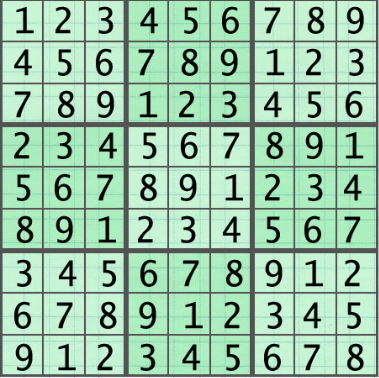
\includegraphics{images/ZakladniGrid.PNG}
    \label{fig:ZakladniGrid}
\end{figure}

\subsubsection{Copy Array Segment}
Metoda kopíruje části permutace a vloží zkopírovanou část na nové misto v poli.

\begin{small}
\begin{lstlisting}
private void copyArraySegment(int resourceRow, int resourceColumn, int resultRow, int resultColumn, int segmentLength) {
        for (int i = 0; i < segmentLength; i++) {
            // Vlozim cast permutace na jine misto
            this.matrix[resultRow][resultColumn + i] = this.matrix[resourceRow][resourceColumn + i];
        }
    }
\end{lstlisting}
\end{small}
Metoda na vstupu dostane číslo řádku, ze kterého bude kopírovat část permutace (resourceRow), číslo sloupce, ze kterého bude kopírovat část permutace (resourceColumn), číslo řádku, do kterého bude vkládat zkopírovanou část permutace (resultRow), číslo sloupce, do kterého bude vkládat zkopírovanou část permutace (resultColumn) a délku části permutace, kterou bude kopírovat (segmentLength).

\subsubsection{Row Permutation}
Metoda pomocí metody Copy ArraySegment rovná za sebou v určitém pořadí zkopírované části o délce 3 políček permutace a pak je vkláda na určitý řádek podle pravidel sudoku\\
Napriklad: 1 2 3 | 4 5 6 | 7 8 9\\
. \hspace{1.6cm} 4 5 6 | 7 8 9 | 1 2 3 atd.

\subsubsection{Move Permutation}
Metoda na vstupu dostane číslo řádku, ze kterého bude přesouvat část permutace (resourceRow) a číslo řádku, do kterého bude část permutace přesouvat (resultRow). Metoda přesune permutaci kromě jejího prvního čísla z počátečního řádku (resultRow) na jiný řádek (resultRow) a potom dosadí první číslo na poslední pozici v řádku.\\
Priklad:  1 2 3 | 4 5 6 | 7 8 9\\
. \hspace{1.15cm}          2 3 4 | 5 6 7 | 8 9 1\\
. \hspace{1.15cm}          3 4 5 | 6 7 8 | 9 1 2 atd.\\
\\
\begin{small}
\begin{lstlisting}
private void movePermutation(int resourceRow, int resultRow) {
        for(int i = 0; i < matrix[resultRow].length - 1; i++) {
            matrix[resultRow][i] = matrix[resourceRow][i + 1];
        }
        matrix[resultRow][8] = matrix[resourceRow][0];
    }
\end{lstlisting}
\end{small}

\subsubsection{Generate}
Metoda s použitím předchozích metod movePermutation a rowPermutation vytvoří mřížku s řešením sudoku.

\section{Řešení 2}
Řešení číslo 2 dokáže vygenerovat všechny možné řešení sudoku narozdíl od řešení číslo 1, spočívá v tom, že do mřížky 9x9 dosadíme tři čtverce 3x3, ve kterých je každé číslo 1-9 právě jednou, po diagonále z levého horního rohu do pravého dolního rohu jako na obrázku \ref{fig:Sudoku3ctverce}. Dosadíme tyto čtverce po diagonále, protože čtverci nemají společný žádný řádek ani sloupec a nemusíme přemíslet o tom jak do čtverce dosadíme čísla 1-9. Potom dosadíme čísla do prázdných políček podle pravidel sudoku, tak že zkontrolujeme, že v řádku, ve sloupci a čtverci 3x3, do kterých dosazujeme číslo je každé číslo právě jednou. Pro získání náhodného řešení třídu SudokuRandomSolutionGenerator.Tímto řešením problému jsem se inspiroval zde \cite{Reseni2}.

\begin{figure}[h!]
    \centering
    \caption{Sudoku 3 Čtverce}
    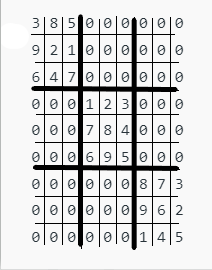
\includegraphics{images/Sudoku3ctverce1.PNG}
    \label{fig:Sudoku3ctverce}
\end{figure}

\subsection{Sudoku Random Solution Generator}
Tato třída vytvoří všechna možná řešení sudoku. Využívá při tom již dříve zmíněnou třídu PermutationGenerator \ref{PermutationGenerator} a třídu CellCoordinates. Ještě využívá metody: generateSquare, checkRow, checkColumn, checkSquare, fillCell, fillSquares, fillCells a generate.

\label{GenerateSquare}\subsubsection{Generate Square}
Metoda vytvoří čtverec 3x3, tak že každé číslo v něm bude právě jednou. Metoda na vstupu dostane souřadnice levého horního rohu čtverce 3x3 ve čtverci 9x9, tam budeme chtít vytvořený čtverec 3x3 vložit.

\begin{small}
\begin{lstlisting}
private void generateSquare(int SquareLeftCornerX, int SquareLeftCornerY) {
        // Ziskam permutaci
        pg.generate();
        for(int i = 0; i < 3; i++) {
            // Vkladam permutaci do ctverce 3x3 po radcich
            this.matrix[SquareLeftCornerX][SquareLeftCornerY + i] = pg.permutation[0 + i];
            this.matrix[SquareLeftCornerX + 1][SquareLeftCornerY + i] = pg.permutation[3 + i];
            this.matrix[SquareLeftCornerX + 2][SquareLeftCornerY + i] = pg.permutation[6 + i];
        }
    }
\end{lstlisting}
\end{small}

Metoda pomocí třídy PermutationGenerator \ref{PermutationGenerator} získám permutaci, kterou od levého horního rohu po řádcích vložím do čtverce 3x3.

\label{CheckRow}\subsubsection{Check Row}
Metoda na vstupu dostane číslo řádku a číslo, které chceme do nej dosadit. Metoda zkontroluje, jestli můžeme dosadit do řádku číslo, tak že porovná číslo na vstupu s čísly, které již v řádku jsou. Pokud najdeme nějaké číslo, kterému se dosazované číslo rovná, metoda vrátí false, jinak vrátí true.

\begin{small}
\begin{lstlisting}
private boolean checkRow(int Number, int Row) {
        // Prochazim cely radek
        for (int i = 0; i < this.matrix.length; i++) {
            if (Number == this.matrix[Row][i])
                return false;
        }
        return true;
    }
\end{lstlisting}
\end{small}

\label{CheckColumn}\subsubsection{Check Column}
Tato metoda funguje a vypadá skoro stejně jako metoda checkRow \ref{CheckRow}, jenom místo řádku (Row) je v této metodě sloupec (Column).

\label{CheckSquare}\subsubsection{Check Square}
Metoda na vstupu dostane souřadnice políčka a číslo, které chceme do nej dosadit. Metoda zkontroluje, jestli může dosadit do políčka číslo, tak že porovná číslo na vstupu s čísly, které již ve čtverci 3x3 jsou. Pokud najde nějaké, kterému se číslo rovná, vrátí false, jinak vrátí true.

\begin{small}
\begin{lstlisting}
private boolean checkSquare(int Number, int X, int Y) {
        // Vytvorim instanci policka se souradnicemi X, Y
        CellCoordinates cell = new CellCoordinates(X, Y);
        // Ziskam souradnice leveho horniho rohu ctverce 3x3
        CellCoordinates squareLeftCorner = cell.mySquare();

        // Od levehho horniho rohu prochazim ctverec 3x3 po radcich
        for (int i = squareLeftCorner.Row; i < squareLeftCorner.Row + 3; i++) {
            for (int j = squareLeftCorner.Column; j < squareLeftCorner.Column + 3; j++) {
                if (Number == this.matrix[i][j])
                    return false;
            }
        }
        return true;
    }
\end{lstlisting}
\end{small}
Na vstupu metoda dostane souřadnice políčka, do kterého chceme dosadit číslo, ale my nevíme v jakém z 9 čtverců 3x3 se nachází naše políčko a také neznáme souřadnice levého horního rohu (to potřebujeme pro to abychom dokázali lehce zkontrolovat čtverec 3x3), ve kterém se nachazí políčko, které chceme zkontrolovat. Abychom zjistili souřadnice levého horního rohu čtverce, kde se nachází kontrolované políčko, využijeme třídy CellCoordinates \ref{CellCoordinates}.

\label{FillCell}\subsubsection{Fill Cell}
Metoda na vstupu dostane souřadnice prázdného políčka. Metoda vyplní prázdné políčko vhodným číslem dle pravidel sudoku: provedeme kontrolu řádku, sloupce a čtverce 3x3.

\begin{small}
\begin{lstlisting}
private void fillCell(int cellRow, int cellColumn) {
        int newNumber = 0;
        boolean wrongNumber = true;

        // Dokud nemame vhodne cislo a zaroven dosazovane cislo
        // neni vetsi nez 9
        while (wrongNumber && (newNumber < 9)) {
            wrongNumber = false;
            // Vygenerujeme nove cislo zvysenim o 1
            newNumber = newNumber + 1;
            // Zkontrolujeme, jestli cislo lze dosadit do radku,
            // sloupce a ctverce 3x3
            if (!(checkRow(newNumber, cellRow)) || (!checkColumn(newNumber, cellColumn)) || (!checkSquare(newNumber, cellRow, cellColumn)))  {
               wrongNumber = true;
            }
        }
        // Vyplnim policko vybranym cislem
        this.matrix[cellRow][cellColumn] = newNumber;
    }
\end{lstlisting}
\end{small}

Metoda dosazuje do políčka postupně čísla od 1 do 9 (a zde nastal problém v programu \ref{Problem}) a pomocí metod checkRow \ref{CheckRow}, checkColumn \ref{CheckColumn} a checkSquare \ref{CheckSquare} zkontroluje jestli tam to číslo může vložit.

\label{FillSquares}\subsubsection{Fill Squares}
Metoda pomocí metody Generate Square \ref{GenerateSquare} vloží 3 čtverce 3x3 po diagonále jako na obrázku \ref{fig:Sudoku3ctverce}

\label{FillCells}\subsubsection{Fill Cells}
Metoda vyplni vsechna neobsazena policka spravnymi cisly dle pravidel sudoku.

\begin{small}
\begin{lstlisting}
private void fillCells() {
        // Prochazim cele pole 9x9 od leveho horniho rohu
        for(int i = 0; i < this.matrix.length; i++) {
            for(int j = 0; j < this.matrix[i].length; j++) {
                if (this.matrix[i][j] == 0) {
                    fillCell(i, j);
                }
            }
        }
    }
\end{lstlisting}
\end{small}

Metoda projde celé pole 9x9 od levého horního rohu a když najde políčko, které se rovná 0, tak pomocí metody Fill Cell \ref{FillCell} políčko zaplní číslem 1-9.

\subsubsection{Generate}
Pomocí metod Fill Squares \ref{FillSquares} a Fill Cells \ref{FillCells} vyplní mřížku sudoku 9x9 řešením.

\label{CellCoordinates}\subsection{Cell Coordinates}
Třída dokáže zjistit v jakém čtverci 3x3 se nachází naše políčko a zjistí souřadnice levého horního rohu čtverce 3x3, ve kterém je naše políčko. Třída má jeden parametrický konstruktor, který dostane souřadnice našeho políčka.

\subsubsection{My Square}
Metoda vrací souřadnice levého horního rohu čtverce 3x3, ve kterém se nachazí naše políčko. Pokud si od bodu [0][0] pole 9x9 označíme každy třetí řádek a sloupec včetně řádku 0 a sloupce 0, tak průsečíky těchto řádku a sloupců budou horní levý rohy čtverce 3x3. 

\begin{small}
\begin{lstlisting}
public CellCoordinates mySquare() {
        int cornerColumn = 0;
        int cornerRow = 0;

        // Najdeme sloupec, ve kterem se nachazi
        // levy horni roh ctverce
        if (this.Column / 3 == 0) {
            cornerColumn = 0;
        }
        else if (this.Column / 3 == 1) {
            cornerColumn = 3;
        }
        else if (this.Column / 3 == 2) {
            cornerColumn = 6;
        }

        //Najdeme radek, ve kterem se nachazi
        //levy horni roh ctverce
        if (this.Row / 3 == 0) {
            cornerRow = 0;
        }
        else if (this.Row / 3 == 1) {
            cornerRow = 3;
        }
        else if (this.Row / 3 == 2) {
            cornerRow = 6;
        }

        return new CellCoordinates(cornerRow, cornerColumn);
    }
\end{lstlisting}
\end{small}

Metoda vydělí souřadnice políčka, aby zjistila, ve které ze 3 částí pole 9x9 se políčko nachází. Pokud se podíl bude rovnat 0 políčko se nachází v 1. části atd.

\label{Problem}\section{Problem}
Když metoda Fill Cell \ref{FillCell} zkouší dosadit čísla do políčka postupně od 1 do 9, tak někdy může nastat situace, že by bylo lepší dosadit do políčka větší číslo než menší, ale jelikož metoda zkouší dosazovat čísla od nejmenšího do největšího, tak pokud se do toho políčka menší číslo hodí, tak větší číslo nemůže být dosazeno dříve. Kvůli tomuto problému mi bohužel 2. řešení nefunguje.
\chapter{Mazání čísel}
Zde se mažou náhodně čísla z pole s řešením sudoku a následně vzniká hotová hra sudoku. Čísla se z pole mažou pomocí třídy SudokuGameGenerator. 

\section{Sudoku Game Generator}
Třída vzmaže čísla z pole s řešením a tím vytvoří hotovou hru sudoku pomocí metod: remove, generateLevel, generate9 a print.

\label{Remove}\subsubsection{Remove}
Metoda odstraňuje čísla z náhodných políček sudoku. Metoda na vstupu dostane číslo, které určuje počet číslic, které odstraníme.

\begin{small}
\begin{lstlisting}
public void remove(int Number) {
        // Urcuje pocet cislic, ktere vymazeme z pole s resenim sudoku
        int removedNumber = Number;
        // Dokud nebude pocet vymazanych cislic 0
        while (removedNumber != 0) {
            // Vygeneruji nahodne cislo od 0-81
            int cellNumber = this.r.nextInt(81);
            // Zjistim radek vygenerovaneho cisla
            int rowNumber = cellNumber / 9;
            // Zjistim sloupec vygenerovaneho cisla
            int columnNumber = cellNumber % 9;
            if (matrix[rowNumber][columnNumber] != 0) {
                matrix[rowNumber][columnNumber] = 0;
                removedNumber--;
            }
        }
    }
\end{lstlisting}
\end{small}

Vygeneruje se náhodné číslo od 0-81 a to číslo je číslo políčka v 2D poli (cellNumber), potom zjistí řádek (rowNumber) vygenerovaného čísla pomocí dělení náhodného čísla 9 (51/9 = 5), pak pomocí operace modulo zjistí sloupec (columnNumber) náhodného čísla (51 \% 9 = 6) políčko, na souřadnicích rowNumber a columnNumber, se přepíše na 0.

\label{GenerateLevel}\subsubsection{Generate Level}
Metoda dostane na vstupu textový řetězec, který určuje obtížnost. Metoda určuje kolik čísel máme vymazat ze sudoku.

\begin{small}
\begin{lstlisting}
private int generateLevel(String difficulty) {
        if (difficulty.equals("Easy")) {
            // Vygeneruje cislo v rozmezi 41 - 48
            return 41 + this.r.nextInt(8);
        } else if (difficulty.equals("Medium")) {
            // Vygeneruje cislo v rozmezi 49 - 56
            return 49 + this.r.nextInt(8);
        } else if (difficulty.equals("Hard")) {
            // Vygeneruje cislo v rozmezi 57 - 64
            return 57 + this.r.nextInt(8);
        } else {
            return 0;
        }
    }
\end{lstlisting}
\end{small}

\label{Generate9}\subsubsection{Generate9}
Metoda dostane na vstupu textový řetězec, který určuje obtížnost. Metoda pomocí metod Generate Level \ref{GenerateLevel} a Remove \ref{Remove} vygeneruje sudoku 9x9.

\begin{small}
\begin{lstlisting}
public void generate9(String difficulty) {
        // Vygeneruji reseni 9x9 sudoku
        ssg9.generate9();
        // Nastavim pole s resenim sudoku do pole teto tridy
        this.matrix = ssg9.matrix;
        System.out.println(difficulty);
        int level = generateLevel(difficulty);
        remove(level);
        print();
    }
\end{lstlisting}
\end{small}

\subsubsection{Print}
Metoda pomocí metody Generate9 \ref{Generate9} a knihovny Swing vypise cele sudoku 9x9 do graficke sceny. Inspiroval jsem se zde \cite{GUI}.

\begin{small}
\begin{lstlisting}
public void print() {
        // Pojmenuji si grafickou scenu
        JFrame f = new JFrame("Sudoku");
        // Vytvorim si graficke textove pole 9x9
        JLabel board[][] = new JLabel[9][9];
        // Vytvorim si mrizkovanou tabulku
        JPanel Board = new JPanel(new GridLayout(9, 9));
        // Prochazim pole od leveho horniho rohu
        for (int i = 0; i < 9; i++) {
            for (int j = 0; j < 9; j++) {
                // Pokud se policko rovna 0 v grafickem poli se na tomto policku nezobrazi nic
                if (this.matrix[i][j] == 0) {
                    board[i][j] = new JLabel("");
                }
                else {
                    // String.valueOf(arr[i][j]) - nastavim int z policka na hodnotu String
                    // Vlozim int v hodnote String do grafickeho policka
                    board[i][j] = new JLabel(String.valueOf(this.matrix[i][j]));
                }
                    // Nastavim si barvu mrizky
                    board[i][j].setBorder(BorderFactory.createLineBorder(Color.PINK));
                    // Nastavim si styl a velikost pisma
                    Font font = new Font("Arial", Font.PLAIN, 20);
                    board[i][j].setFont(font);
                    // Nastavim barvu popredi
                    board[i][j].setForeground(Color.BLACK);
                    // Nastavim barvu pozadi
                    board[i][j].setBackground(Color.BLACK);
                    // Vycentruji graficke pole
                    board[i][j].setHorizontalAlignment(JTextField.CENTER);
                    // Pridam graficke pole do grafickeho okna
                    Board.add(board[i][j]);
            }
        }
        // Pridam graficke okno na grafickou scenu
        f.add(Board);
        // Nastavim rozmery graficke sceny
        f.setSize(400, 400);
        // Nastavim viditelnou scenu
        f.setVisible(true);}
\end{lstlisting}
\end{small}
\chapter{Závěr}
Řešení číslo 1 se mě povedlo a program funguje, tak jak má. I když jsem v zadání neměl grafické rozhraní, tak se mi podařilo ho udělat za co jsem neskutečně rád. Bohužel se nepodařilo zprovoznit řešení číslo 2, kvůli problému \ref{Problem} s dosazováním čísel od nejmenšího po největší. Dle mého názoru můj 1 velký projekt dopadl velmi dobře, hlavně jsem rád za to, že mi něco funguje.
\bibliographystyle{plain}
\bibliography{ref}

\end{document}
